\subsection{Specifica dei canali di comunicazione}
\label{sct:specif_meccanismi_intro}
\begin{figure}[!t]
  \begin{subfigure}[b]{.5\textwidth}
    \centering
    %% \resizebox{\columnwidth}{!}{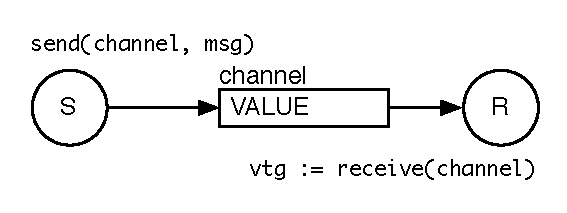
\includegraphics{abstract_sym.pdf}}
    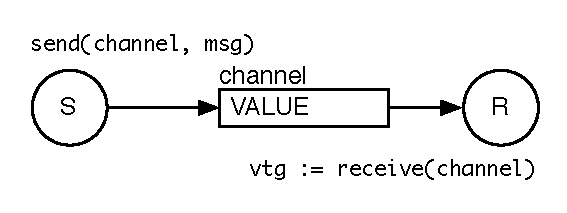
\includegraphics[scale=.5]{abstract_sym.pdf}
    \caption{Canale simmetrico}
    \label{fig:abstract_channel_sym}
  \end{subfigure}
  \begin{subfigure}[b]{.5\textwidth}
    \centering
    %% \resizebox{\columnwidth}{!}{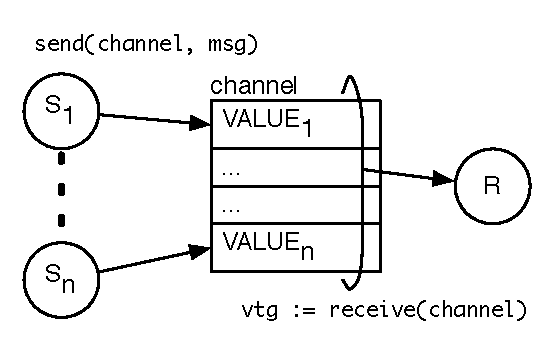
\includegraphics{abstract_asym.pdf}}
    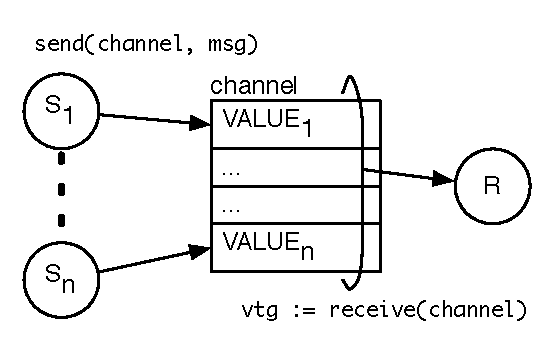
\includegraphics[scale=.5]{abstract_asym.pdf}
    \caption{Canale asimmetrico in ingresso}
    \label{fig:abstract_channel_asym}
  \end{subfigure}
  \caption[Canali di comunicazione tra processi]{Rappresentazione astratta di canali con grado di asincronia unitario}
  \label{fig:abstract_channels}
\end{figure}

%% >>>> INTRODUZIONE
%% ---> TODO
%% Si desidera implementare meccanismi di \emph{fast} message passing, in particolare canali di comunicazione simmetrici e asimmetrici in ingresso con grado di asincronia 1 e tipo di dato ``riferimento''. Si applica la copia del valore del messaggio nel canale.

%%Al fine di poter offrire un supporto efficiente ai paradigmi di programmi paralleli caratterizzati da grana fine sia nelle computazioni nei processi che nelle comunicazioni tra processi \`e stata studiata l'implementazione di meccanismi di \emph{fast} message passing nel CMP \tile. Meccanismi di questo tipo sono caratterizzati da una bassa latenza di comunicazione, 

%% Le forme di comunicazione che sono espresse da tali meccanismi sono sufficienti per fornire il supporto dei principali paradigmi di programmazione parallela. Il grado di asincronia unitario risulta sufficiente per le forme di parallelismo e consente minori overhead nell'implementazione dei meccanismi rispetto a gradi di asincronia maggiori di uno.

%% >>>> DESCRIZIONE DEI MECCANISMI
Con canale di comunicazione si intende il collegamento logico tramite il quale due o pi\`u processi comunicano. L'astrazione di canale come meccanismo primitivo di scambio di informazioni tra processi viene fornita dal supporto a tempo di esecuzione della nostra libreria. Il canale \emph{simmetrico} \`e un oggetto che mette in comunicazione un processo mittente con un processo destinatario, consentendo l'invio di messaggi dal processo mittente al processo destinatario. Un canale \emph{asimmetrico in ingresso} \`e un oggetto che mette in comunicazione pi\`u processi mittenti con un singolo processo destinatario, consentendo a ciascun mittente l'invio di messaggi al processo destinatario. Il destinatario riceve i messaggi in modo non deterministico e senza saperne la provenienza, a meno di comunicazioni esplicite. 

Per entrambi i canali sono definite due primitive di comunicazione, quella di invio e quella di ricezione le quali sono usate rispettivamente dal processo mittente e dal processo destinatario del canale di comunicazione. Si considera la seguente dichiarazione C delle primitive:
\begin{lstlisting}[morekeywords={ch_sym_t, ch_asym_t}]
void sym_send(ch_sym_t *ch_descr, const void *msg)
void *sym_receive(ch_sym_t *ch_descr)

void asym_send(ch_asym_t *ch_descr, const void *msg, int rank)
void *asym_receive(ch_asym_t *ch_descr)
\end{lstlisting}
Ad ogni primitiva viene quindi passato, come primo parametro, il descrittore di canale come riferimento ad una struttura dati allocata in memoria condivisa. Non viene usata la tecnica zero-copy in quanto non \`e applicabile all'implementazione che fa uso della UDN. La primitiva di invio ha come secondo parametro il valore del messaggio, quella di ricezione ritorna il valore letto dal canale come valore di ritorno, il valore del messaggio \`e copiato prima nel canale poi nella variabile targa. Nel caso asimmetrico \`e necessario specificare alla primitiva di invio l'identificatore del mittente all'interno del canale, ci\`o \`e necessario per l'implementazione, come spiegato nelle sezioni successive per entrambi i supporti.

%% >>>> SPECIFICA PRIMITIVE DI COMUNICAZIONE
Si considera il seguente comportamento ad alto livello delle due forme di comunicazione con il grado di asincronia considerato:
%% Si considerano le seguenti specifiche del comportamento della primitiva di invio su un canale simmetrico con grado di asincronia unitario:
\begin{description}
\item [canale simmetrico con grado di asincronia unitario] prevede che il processo mittente possa inviare fino ad un messaggio senza attendere che il destinatario lo abbia ricevuto. Nel caso in cui il mittente intenda inviare un secondo messaggio senza che il destinatario abbia ricevuto quello precedente occorre che il mittente attenda la ricezione da parte del destinatario.
\item [canale asimmetrico in ingresso con grado di asincronia unitario] \hfill ogni processo mittente pu\`o inviare fino ad un messaggio senza attendere che il destinatario lo abbia ricevuto. Nel caso in cui un generico mittente intenda inviare un secondo messaggio senza che il destinatario abbia ricevuto il messaggio precedentemente inviato dal quello specifico mittente, occorre che tale mittente attenda la ricezione da parte del destinatario del messaggio precedente. 
\end{description}
Per quanto riguarda il comportamento del ricevente di un canale asimmetrico, non si impone una specifica politica di ricezione. Il comportamento che pu\`o essere considerato naturale \`e la ricezione FIFO dei messaggi inviati dai mittenti, tuttavia tale funzionamento non \`e imposto. Si pu\`o infatti parlare del canale asimmetrico in ingresso come un caso particolare di comportamento non deterministico del destinatario nella ricezione da pi\`u canali simmetrici.

\begin{lstlisting}[
    float = b,
    caption = {Descrizione astratta del protocollo di comunicazione per un canale simmetrico con grado di asincronia 1}, 
    label = lst:abstract_sym_protocol,
    morekeywords={msg, vtg, ready, acknowledgement, sender, receiver}
]
send ::
  wait until acknowledgement signal is received
  send the message to receiver and
    reset acknowledgement flag and
    signal ready to the receiver
  
receive ::
  wait until ready signal is received
  copy the message received from sender into vtg and
    reset ready flag and
    signal acknowledgement to the sender
\end{lstlisting}
Nelle sezioni successive verranno descritte le implementazioni dei due tipi di canale che sfruttano supporti architetturali diversi. I protocolli di comunicazione che costituiscono l'implementazione con i diversi supporti fanno riferimento al protocollo usato al livello firmware per la comunicazione di due unit\`a di elaborazione indipendente dal tempo. Tale protocollo \`e chiamato nel seguito Rdy-Ack. Descriviamo qui, in modo astratto, le azioni dei processi comunicanti definite dal protocollo che assicurano la correttezza della comunicazione, ovvero: 
\begin{itemize}
\item non si verifica mai la perdita di un messaggio,
\item se il/un processo mittente invia un messaggio allora prima o poi il processo destinatario lo deve ricevere,
\item se il processo destinatario riceve un messaggio allora prima o poi il processo mittente che ha effettuato l'invio di quel messaggio deve essere in grado di inviarne un altro.
\end{itemize}
%% >>>> DESCRIZIONE DEL PROTOCOLLO
Per il canale simmetrico si hanno le azioni delle due entit\`a descritte nel codice~\ref{lst:abstract_sym_protocol}. Il canale asimmetrico in ingresso ha protocollo simile, in quanto pu\`o essere visto come costituito da tanti canali simmetrici Rdy-Ack quanti sono i mittenti, dove ogni canale collega un mittente al destinatario. Il comportamento dell'invio di un messaggio \`e esattamente lo stesso di quello adottato nel canale simmetrico, mentre la ricezione ha l'onere di scegliere in modo non deterministico un canale da cui ricevere tra i canali pronti.



%% che il \emph{mapping} delle applicazioni parallele considerate nell'architettura \`e di \emph{tipo esclusivo}, ovvero esiste una corrispondenza biunivoca tra ogni processo dell'applicazione e il processore della macchina che lo esegue. 
%% ---> MOTIVAZIONI
